% mainfile: ../../../../master.tex
\subsection{RNA Quantification with Qubit\texttrademark~ RNA BR Assay}
% The part of the label after the colon must match the file name. Otherwise,
% conditional compilation based on task labels does NOT work.
\label{task:20180301_cj3}
\tags{lab,rna,qnt}
\authors{cj}
%\files{}
%\persons{}
\sidenote{Qubit\texttrademark RNA BR Assay kit; \texttt{LOT: 1924395} opened by me on 20180210.}

\begin{figure}[H] % position of the figure 
    \centering
    \caption{Illustration for the Qubit\texttrademark~ RNA BR assay}
    \label{fig:20180301_Qubit_RNA_BR}
    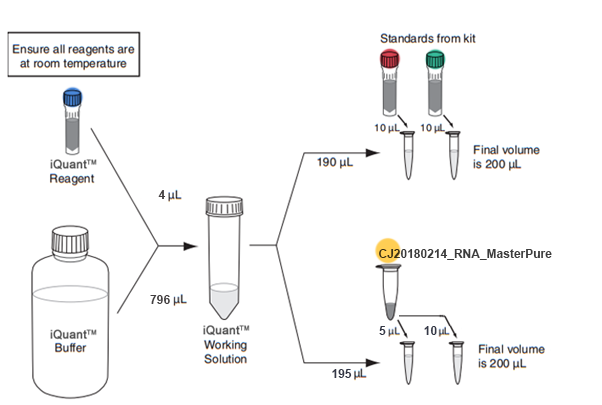
\includegraphics[width=0.8\textwidth]{graphics/schemas/20180215_Qubit_RNA_BR.png}
\end{figure}

\sidenote{I repeated exactly the same as I did on the 20180215 and on the 20180227.}

\begin{table}[H]
\caption{Total RNA quantities in samples measured with Qubit\texttrademark~ RNA BR Assay Kit}
\label{tab:20180215_rna_qnt}
\centering
\begin{tabular}{l r r r r}
\toprule
Sample ID & \textmu g/mL & $V_f$ (mL) & m (\textmu g) & m (ng) \\ \midrule
\texttt{CJ20180301\_RNA\_AllPrep\_5} & 14.4 & 0.080 & 1.152 & 1152.0 \\
\texttt{CJ20180301\_RNA\_AllPrep\_10} & 14.0 & 0.080 & 1.120 & 1120.0 \\
\midrule
\texttt{CJ20180301\_RNA\_AllPrep\_5} & 14.3 & 0.080 & 1.144 & 1144.0 \\
\texttt{CJ20180301\_RNA\_AllPrep\_10} & 14.4 & 0.080 & 1.152 & 1152.0 \\
\texttt{CJ20180301\_RNA\_AllPrep\_5} & 14.0 & 0.080 & 1.120 & 1120.0 \\
\texttt{CJ20180301\_RNA\_AllPrep\_10} & 14.4 & 0.080 & 1.144 & 1144.0 \\
\bottomrule
\end{tabular}
\end{table}

In table \ref{tab:20180215_rna_qnt}, the two first rows contain measures obtained with the last calibration while the four last rows contain values measured with a new calibration. I must say I am impressed by the consistency of these results (maybe because the kit is very new). 

According to these measurements and knowing that the total volume of RNase-free water used to elute the RNA was 80~\uL, my RNA yield is 1.120 ug, which is enough for metatranscriptomics. 

And these time, the quantity of RNA isolated is higher than the quantity of DNA, which is what is expected. Therefore, when using the AllPrep Mini Kit for DNA and RNA isolation, I will use the gentle bead beating step for homogeneisation.

